%\documentclass[tikz, border=5pt]{standalone}
\begin{document}
	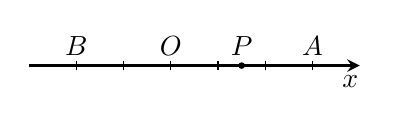
\begin{tikzpicture}[scale=0.6]
		% 绘制主水平线
		\draw[->, >=stealth, line width=1pt] (-1,0) -- (6,0);
		
		% 6个小竖线标记点(从左到右)
		\draw (0,0.1) -- (0,-0.1);    % 第一个竖线标记
		\draw (1,0.1) -- (1,-0.1);    % 第二个竖线标记
		\draw (2,0.1) -- (2,-0.1);    % 第三个竖线标记
		\draw (3,0.1) -- (3,-0.1);    % 第六个竖线标记
		\draw (4,0.1) -- (4,-0.1);    % 第四个竖线标记
		\draw (5,0.1) -- (5,-0.1);    % 第五个竖线标记

		% 实心圆点P
		\fill (3.5,0) circle (2pt) node[above] {$P$};  % 带标签的实心点
		
		% 为竖线标记添加标签
		\node[above] at (0,0) {$B$};
		\node[above] at (5,0) {$A$};
		\node[above] at (2,0) {$O$};
		\node[below] at (5.8,0) {$x$};
		
	\end{tikzpicture}
\end{document}

